\documentclass[11pt]{article}
\usepackage[T1]{fontenc}
\usepackage{lmodern}
\usepackage[margin=1in]{geometry}
\usepackage{amsmath,amssymb,amsthm,mathtools}
\usepackage{booktabs,longtable,array}
\usepackage{graphicx,xcolor,microtype,enumitem}
\usepackage{fancyhdr}
\usepackage{xurl}
\definecolor{navy}{HTML}{17324D}
\definecolor{teal}{HTML}{126B72}
\usepackage[colorlinks=true,linkcolor=navy,citecolor=teal,urlcolor=teal,
  pdftitle={Cyclotomic Obstructions and Optimal Truncation for the Herglotz--Zagier Function},
  pdfauthor={Research continuation prepared for Vladimir Reshetnikov}]{hyperref}
\pagestyle{fancy}
\fancyhf{}
\fancyhead[L]{\small\textsc{Herglotz--Zagier research continuation}}
\fancyhead[R]{\small ProveIt}
\fancyfoot[C]{\thepage}
\setlength{\headheight}{14pt}
\setlength{\emergencystretch}{2em}
\makeatletter
\renewcommand{\l@section}[2]{%
  \ifnum\c@tocdepth>\z@
    \addpenalty\@secpenalty\vskip4pt
    {\bfseries\@dottedtocline{1}{0em}{1.6em}{#1}{#2}}%
  \fi}
\makeatother
\setlist[itemize]{topsep=4pt,itemsep=3pt}
\setlist[enumerate]{topsep=4pt,itemsep=3pt}
\numberwithin{equation}{section}
\newtheorem{theorem}{Theorem}[section]
\newtheorem{lemma}[theorem]{Lemma}
\newtheorem{proposition}[theorem]{Proposition}
\newtheorem{corollary}[theorem]{Corollary}
\theoremstyle{definition}
\newtheorem{definition}[theorem]{Definition}
\newtheorem{example}[theorem]{Example}
\theoremstyle{remark}
\newtheorem{remark}[theorem]{Remark}
\newcommand{\Q}{\mathbb Q}
\newcommand{\R}{\mathbb R}
\newcommand{\C}{\mathbb C}
\newcommand{\Z}{\mathbb Z}
\newcommand{\E}{\mathbb E}
\newcommand{\Pcal}{\mathcal P}
\newcommand{\Bcal}{\mathcal B}
\newcommand{\Acal}{\mathcal A}
\newcommand{\Vcal}{\mathcal V}
\newcommand{\Lam}{\mathcal L}
\newcommand{\cl}[1]{\langle #1\rangle}
\newcommand{\Fone}{F(1)}
\DeclareMathOperator{\Li}{Li}
\DeclareMathOperator{\Cl}{Cl}
\DeclareMathOperator{\Gal}{Gal}
\DeclareMathOperator{\rank}{rank}
\DeclareMathOperator{\Span}{span}
\DeclareMathOperator{\dist}{dist}
\DeclareMathOperator{\Reg}{Reg}
\DeclareMathOperator{\Rea}{Re}
\DeclareMathOperator{\Ima}{Im}

\title{\color{navy}Cyclotomic Obstructions and Optimal Truncation\\
for the Herglotz--Zagier Function\\[5pt]
\large All-conductor rank theorems, exact reduction criteria,\\
and corrections to the Polylogarithms drafts}
\author{A research continuation prepared for Vladimir Reshetnikov\\
\small ProveIt / Analysis / Polylogarithms}
\date{8 October 2026 (UTC)}

\begin{document}
\maketitle
\begin{abstract}
We determine all rational linear relations among the cyclotomic exterior
symbols attached to the Herglotz--Zagier function, for every conductor.
For $G_q=(\Z/q\Z)^\times/\{\pm1\}$, the only relations among
$\beta_q(a)$ are inverse symmetry: a coefficient vector is in the kernel
exactly when $c_a=c_{a^{-1}}$. Consequently the rank is
$(|G_q|-|G_q[2]|)/2$, and $\beta_q(a)=0$ exactly when
$a^2\equiv\pm1\pmod q$. The proof uses a positive definite Gram matrix
of cyclotomic logarithms and the nonvanishing of primitive Dirichlet
$L$-values; it does not assume independence of a redundant collection of
cyclotomic units. Combining this theorem with a field-norm separation
argument gives an exact criterion for reduction of $F(p/q)-F(1)$ to
rational-argument dilogarithms in the standard five-term calculus.
It also completely classifies the formal logarithmic and rational-dilogarithmic
reductions of $J(2/q)$.

A second part derives sharp, uniform optimal-truncation laws from the
known Binet--Lambert representation. The least possible truncation error
is $x^{-1/2}e^{-2\pi x}$ times an explicit correction with a periodic
dependence on the integer cutoff. We prove existence and uniqueness of
every cutoff transition, compute its algebraic asymptotics, and isolate
the smaller arithmetic displacement $-(9/10)K2^{-K}$ from an exactly
defined one-frequency reference. Positive-measure bounds yield exact
rational error certificates. A targeted audit corrects false reduction
claims in the repository, an undefined even-denominator derivative sum,
and several regulator normalizations, and gives an explicit counterexample
to a finite-field identity in the inspected 2020 source preprint.
\end{abstract}

\noindent\textbf{Research status.}
All theorems below have mathematical proofs. The executable checks are
supporting evidence and reproducibility aids. Statements about the
\emph{formal} dilogarithm calculus are distinguished throughout from
unproved assertions about arbitrary numerical relations between periods.
The work is an AI-assisted research draft with independent internal audits;
it has not been externally refereed or formally verified in a proof assistant.

\clearpage
{\small\tableofcontents}
\newpage

\section{Scope, results, and relation to the existing drafts}
\label{sec:scope}

The supplied directory contains several related research threads. We
concentrate on the Herglotz--Zagier thread and its links to the dilogarithm,
cyclotomic units, positive integral kernels, and effective computation.
The source snapshot is the ProveIt commit \cite{ProveIt}
\begin{center}\small\ttfamily
c78c7c3dc2fc742a1af9492e47d578b3fb4e01e7.
\end{center}
The principal repository inputs are the reports
\path{herglotz-arithmetic-study}, \path{herglotz-rational-values},
\path{herglotz-bridges}, and \path{herglotz-stark-regulators}, together
with the Binet--Malmsten report. The article also records a few targeted
corrections to adjacent drafts. The source inventory and exact blob hashes
are included in \texttt{data/source\_snapshot.json}; this is a targeted
mathematical audit, not a claim to have checked every formula in every file.

Our point of departure is Radchenko and Zagier's finite dilogarithm
evaluation and their symbol $\beta$, as well as their Binet--Lambert
integral \cite{RZ}. Those constructions are prior work. The new work here
is the complete relation theorem for $\beta$, its reduction consequences,
and the explicit sharp cutoff analysis.

\subsection{The algebraic result}

For $q\ge3$ let $r_\pm(q)$ count the unit residue classes satisfying
$u^2\equiv\pm1\pmod q$. We prove
\begin{equation}\label{eq:rank-intro}
 \dim_\Q\Span\{\beta_q(a):(a,q)=1\}
 =\frac{\varphi(q)-r_+(q)-r_-(q)}4.
\end{equation}
More strongly, every relation is explicitly known. After identifying
$a$ and $-a$, its coefficients must be constant on inverse pairs.
This statement covers composite conductors as well as prime powers.
It avoids a common obstruction to naive arguments: at composite level,
the primitive cyclotomic units need not be independent.

For coprime positive integers $p,q$, the resulting exact test for
\emph{formal rational-dilogarithm reduction} of $F(p/q)-F(1)$ is
\begin{equation}\label{eq:pair-intro}
 p^2\equiv\pm1\pmod q,
 \qquad q^2\equiv\pm1\pmod p,
\end{equation}
where the signs are independent and the condition modulo $1$ is vacuous.
Theorem~\ref{thm:reduction} specifies precisely what is being classified.
In particular, the theorem does not assert the numerical independence of
dilogarithm values that have a nonzero symbol.

The application to
$J(x)=\int_0^1\log(1+t^x)/(1+t)\,dt$ is especially concrete:
\begin{center}
\begin{tabular}{ll}
\toprule
Reduction of $J(2/q)$, $q\ge2$ & Exactly the following denominators\\
\midrule
Products of algebraic logarithms and $\pi^2$ & $q\in\{2,3,5\}$ or $4\mid q$\\
Also allowing rational-argument dilogarithms & $q\in\{2,3,5,6,10\}$ or $4\mid q$\\
\bottomrule
\end{tabular}
\end{center}
The equivalences in this table are in the five-term calculus. Every
positive case is accompanied by an actual analytic evaluation.

\subsection{The analytic result}

Let $F_N(x)$ truncate the Bernoulli--zeta expansion after $N$ even-power
terms, in addition to the $x^{-1}$ term. Its absolute error $R_N(x)$ is
positive and exactly representable by a positive integral. For
$a=2\pi x$ and $\delta=N-\pi x$ bounded, we prove
\begin{equation}\label{eq:sharp-intro}
 R_N(x)=\frac{e^{-2\pi x}}{\sqrt{x}}
 \left(1+\frac{2\delta^2+\delta-5/12}{a}
 +\frac{2\delta^4+\frac23\delta^3-\frac{10}3\delta^2
 -\frac7{12}\delta+\frac{205}{288}}{a^2}
 +O(a^{-3})\right).
\end{equation}
The error in \eqref{eq:sharp-intro} is uniform on each fixed bounded
$\delta$-interval. The best integer cutoff has a rigorously defined
transition sequence. Its first correction depends on
$\dist(\pi x-1/4,\Z)$, so a single constant correction cannot describe the
optimum uniformly.

The arithmetic displacement of a transition is smaller than every
algebraic correction. We define the reference transition exactly before
subtracting it; otherwise an exponentially small term would be hidden by
an algebraically larger remainder. With $K=2N+2$, its leading coefficient
is $-9/10$ (Theorem~\ref{thm:arithmetic-shift}).

\subsection{What is established, and what remains open}

The rank theorem is an unconditional statement in an exterior power of
an algebraic-number group. The reduction theorems are unconditional
statements in the rationalized pre-Bloch group, using standard Bloch-group
descent. Their successful cases yield analytic identities. Their
unsuccessful cases rule out certificates in that calculus, rather than
all conceivable numerical coincidences. The optimal-truncation theorems
are unconditional real asymptotic theorems with specified uniformity.
We make no claim that a literature search establishes worldwide priority
for every consequence; the explicit results and their proofs, rather than
a priority assertion, are the contribution of this continuation.

\section{The Herglotz function and its formal dilogarithm symbol}
\label{sec:formal}

For $x>0$ define
\begin{equation}\label{eq:F-J}
 F(x)=\sum_{n=1}^{\infty}\frac{\psi(nx)-\log(nx)}n,
 \qquad J(x)=\int_0^1\frac{\log(1+t^x)}{1+t}\,dt.
\end{equation}
The series is absolutely convergent, since
$\psi(z)-\log z=-1/(2z)+O(z^{-2})$ on the positive real axis. The
standard relation between the two functions is
\begin{equation}\label{eq:J-F}
 J(x)=F(2x)-2F(x)+F(x/2)+\frac{\pi^2}{12x}.
\end{equation}
The same functions have holomorphic continuations to the slit plane, but
our error estimates will concern positive real arguments.

We use additive notation for a multiplicative group after rationalization:
\[
 \Acal(K)=K^\times\otimes_\Z\Q,
 \qquad \cl{uv}=\cl u+\cl v.
\]
Roots of unity map to zero. Exterior powers below are over $\Q$ unless
otherwise specified.

\begin{definition}[Pre-Bloch group and formal reduction]\label{def:formal}
Let $\Pcal(K)$ be the $\Q$-vector space on symbols $[z]$, $z\in K$, with
$[0]=[1]=0$, modulo the five-term relations. Its differential is
\[
 \partial[z]=\cl z\wedge\cl{1-z}\quad(z\ne0,1),
 \qquad \partial[0]=\partial[1]=0,
 \qquad \Bcal(K)=\ker\partial.
\]
For an invariant dilogarithm element $\xi\in\Pcal(K)$, a
\emph{formal logarithmic reduction} means $\xi=0$ in $\Pcal(K)$.
A \emph{formal rational-dilogarithm reduction} means that $\xi$ belongs
to the image of $\Pcal(\Q)$. Upon evaluation, five-term relations carry
products of algebraic logarithms and rational multiples of $\pi^2$;
these are the terms suppressed by this terminology.
\end{definition}

For a finite Galois number field $K/\Q$, two standard rationalized facts
will be used:
\begin{equation}\label{eq:bloch-facts}
 \Bcal(K)^{\Gal(K/\Q)}=\Bcal(\Q)=0,
 \qquad \partial\Pcal(\Q)=\Lambda^2\Acal(\Q).
\end{equation}
The first is Bloch-group descent and the torsion of the Bloch group of
$\Q$; the second is equivalent to the torsion of $K_2(\Q)$.
These are established algebraic $K$-theory inputs, not new results of this
article; see \cite{Milnor,ZagierDilog}. The same inputs underpin the
symbol argument in \cite[\S7.2]{RZ}.

Let $\zeta_q=e^{2\pi i/q}$ and, for $(a,q)=1$, set
\begin{equation}\label{eq:beta}
 \beta_q(a)=\sum_{k=1}^{q-1}
 \cl{1-\zeta_q^{ak}}\wedge\cl{1-\zeta_q^k}
 \in\Lambda^2\Acal(\Q(\zeta_q)).
\end{equation}
We put $\beta_1=\beta_2=0$. The term $k=0$ is excluded:
there is no multiplicative-group element $\cl0$.
For coprime positive $p,q$, the finite cyclotomic dilogarithm sum for
$F(p/q)-F(1)$ defines a Galois-invariant element $\xi_{p/q}$ with
\begin{equation}\label{eq:delta-xi}
 \partial\xi_{p/q}=\beta_q(p)-\beta_p(q)-\cl p\wedge\cl q.
\end{equation}
One can take $K=\Q(\zeta_{pq})$. We retain this classical normalization
throughout; the rational wedge in \eqref{eq:delta-xi} matters for the
distinction between logarithms and rational dilogarithms.

\begin{lemma}[Elementary symmetries]\label{lem:symmetry}
For every conductor and every invertible residue $a$,
\[
 \beta_q(-a)=\beta_q(a),\qquad
 \beta_q(a^{-1})=-\beta_q(a).
\]
Each $\beta_q(a)$ is Galois invariant.
\end{lemma}
\begin{proof}
The identity $1-\zeta_q^{-ak}=-\zeta_q^{-ak}(1-\zeta_q^{ak})$
proves the first claim after roots of unity are killed. In the sum for
$\beta_q(a^{-1})$, replace $k$ by $ak$ and reverse the exterior factors.
Finally, every Galois automorphism multiplies $k$ by a unit modulo $q$,
permuting the summation set.
\end{proof}

\section{The all-conductor relation theorem}
\label{sec:rank}

The following is the main algebraic theorem.

\begin{theorem}[Complete kernel, every conductor]\label{thm:kernel}
Let $q\ge3$, $G=G_q=(\Z/q\Z)^\times/\{\pm1\}$, and
$(c_a)_{a\in G}\in\Q^G$. Then
\begin{equation}\label{eq:kernel}
 \sum_{a\in G}c_a\beta_q(a)=0
 \quad\Longleftrightarrow\quad
 c_a=c_{a^{-1}}\quad\hbox{for every }a\in G.
\end{equation}
In particular,
\begin{align}
 \beta_q(a)=0&\quad\Longleftrightarrow\quad a^2\equiv\pm1\pmod q,
 \label{eq:zero-beta}\\
 \dim_\Q\Span\{\beta_q(a):a\in G\}
 &=\frac{|G|-|G[2]|}{2}.
 \label{eq:rank-beta}
\end{align}
Choosing one $a$ from each inverse pair $\{a,a^{-1}\}$ with
$a\ne a^{-1}$ gives a basis of the symbol space.
\end{theorem}

The proof is short after the correct positive matrix is identified.
Its use of \emph{all} nontrivial roots, including those of smaller order,
is essential at composite conductor.

\subsection{Cyclotomic logarithms and a positive Gram matrix}

For $1\le k<q$, define the real vector
\begin{equation}\label{eq:vk}
 v_k=\bigl(\log|1-\zeta_q^{ak}|\bigr)_{a\in G}\in\R^G,
 \qquad A_q=\sum_{k=1}^{q-1}v_kv_k^{\mathsf T}.
\end{equation}
The entries are independent of the representative of $a$ modulo sign.
Let $P_b$ be the permutation matrix
$(P_bv)_a=v_{ab}$. Then
\begin{equation}\label{eq:Gram-equiv}
 P_bv_k=v_{bk},\qquad P_bA_qP_b^{\mathsf T}=A_q,
 \qquad P_bA_q=A_qP_b.
\end{equation}

\begin{lemma}[Positive definiteness]\label{lem:positive-Gram}
The vectors $v_k$ span $\R^G$. Hence $A_q$ is positive definite.
\end{lemma}
\begin{proof}
Complexify the regular representation of the finite abelian group $G$.
Each character occurs once. The span of the $v_k$ is $G$-invariant by
\eqref{eq:Gram-equiv}, so it suffices to show a nonzero Fourier component
for every character.

Let $\chi$ be nontrivial and let $f\mid q$ be its primitive Dirichlet
conductor. It is an even character, so $f>2$. Write $\chi^*$ for the
primitive character modulo $f$. Reduction gives a surjection
$G_q\longrightarrow G_f$. For the vector with $k=q/f$, its Fourier
coefficient is a nonzero positive integer multiple of
\begin{equation}\label{eq:log-L}
 \sum_{a\in G_f}\chi^*(a)\log|1-\zeta_f^a|
 =-\frac12\tau(\chi^*)L(1,\overline{\chi^*})\ne0.
\end{equation}
The equality follows by Abel-regularizing
$\log|1-re^{i\theta}|=-\sum_{n\ge1}r^n\cos(n\theta)/n$,
summing over $a$, using the primitive Gauss-sum identity, and letting
$r\uparrow1$. The Gauss sum is nonzero and Dirichlet's nonvanishing
theorem gives $L(1,\overline{\chi^*})\ne0$. This is a standard
cyclotomic-logarithm identity; cf.\ \cite{Washington,Sharifi}.

For the trivial character, choose a prime $\ell\mid q$. If $\ell$ is
odd, use $k=q/\ell$ and
\[
 \sum_{a\in G_\ell}\log|1-\zeta_\ell^a|
 =\tfrac12\log\ell\ne0.
\]
If $\ell=2$, the vector $v_{q/2}$ is the nonzero constant vector
$(\log2)_{a\in G}$. Thus every character component occurs. This proves
the spanning assertion, and
$w^{\mathsf T}A_qw=\sum_k(w^{\mathsf T}v_k)^2>0$ for $w\ne0$.
\end{proof}

\subsection{From exterior symbols to skew matrices}

There is a $\Q$-linear logarithm map
\[
 \ell:\Acal(\Q(\zeta_q))\longrightarrow\R^G,
 \qquad\ell(\cl u)=(\log|\sigma_a(u)|)_{a\in G}.
\]
Composing its exterior square with the passage to the real exterior
power and then identifying $v\wedge w$ with
$vw^{\mathsf T}-wv^{\mathsf T}$ gives a $\Q$-linear map to real skew
matrices. We do \emph{not} assume this map is injective on the whole
exterior power. Its value on \eqref{eq:beta} is explicitly
\begin{equation}\label{eq:skew-image}
 \ell_\wedge(\beta_q(b))
 =P_bA_q-A_qP_b^{\mathsf T}
 =A_q(P_b-P_{b^{-1}}).
\end{equation}

\begin{proof}[Proof of Theorem~\ref{thm:kernel}]
If the left side of \eqref{eq:kernel} vanishes, apply
\eqref{eq:skew-image} and multiply by the invertible matrix $A_q^{-1}$.
We get
\[
 0=\sum_{b\in G}c_b(P_b-P_{b^{-1}})
 =\sum_{b\in G}(c_b-c_{b^{-1}})P_b.
\]
The regular permutation matrices $P_b$ are linearly independent, even
over $\R$: their values on a single coordinate vector are the distinct
coordinate vectors. Therefore $c_b=c_{b^{-1}}$.

Conversely, if these equalities hold, group the sum into inverse pairs
and use Lemma~\ref{lem:symmetry}; self-inverse classes have
$2\beta_q(b)=0$ and hence contribute zero. This proves
\eqref{eq:kernel}. Applying it to a coefficient vector supported at one
class proves \eqref{eq:zero-beta}, and counting nontrivial inverse pairs
proves \eqref{eq:rank-beta} and the basis assertion.
\end{proof}

\begin{remark}[Why the composite case is not a numerical rank claim]
All matrix entries involving logarithms are used only in the proof of
positive definiteness. The conclusion follows from exact character
nonvanishing, not from a numerical determinant. In particular, no lower
bound for a numerically computed singular value is required. The resulting
coordinate model $\beta_q(a)\mapsto P_a-P_{a^{-1}}$ is exact on the
symbol span, even though its derivation used a real logarithm map.
\end{remark}

\subsection{Explicit rank formula and zero conductors}

\begin{corollary}\label{cor:rank-CRT}
For $q\ge3$,
\[
 d(q):=\dim_\Q\Span\{\beta_q(a)\}
 =\frac{\varphi(q)-r_+(q)-r_-(q)}4.
\]
Write $q=2^e\prod_{j=1}^s p_j^{e_j}$ with distinct odd primes $p_j$.
Then
\[
 r_+(q)=2^s\begin{cases}1&e=0,1,\\2&e=2,\\4&e\ge3,\end{cases}
\]
and $r_-(q)=0$ if $e\ge2$ or some $p_j\equiv3\pmod4$; otherwise
$r_-(q)=2^s$.
\end{corollary}
\begin{proof}
The self-inverse elements of $G_q$ are the sign classes of roots of
$u^2=1$ or $u^2=-1$. These two sets are disjoint for $q>2$, and every
sign class has two representatives. Thus
$|G_q[2]|=(r_++r_-)/2$. The stated root counts follow from the Chinese
remainder theorem and the elementary square-root counts at prime powers.
\end{proof}

\begin{corollary}[Complete list of identically zero conductors]
\label{cor:zero-conductors}
With the conventions at $q=1,2$, the function $\beta_q$ is identically
zero exactly for
\begin{equation}\label{eq:zero-conductors}
 q\in\{1,2,3,4,5,6,8,10,12,24\}.
\end{equation}
\end{corollary}
\begin{proof}
The condition is that $G_q$ have exponent at most $2$. Projecting to
each odd prime-power factor forces that factor to be $3$ or $5$ to the
first power, since its unit group is cyclic and has order dividing $4$.
The $2$-part is at most $8$: the square of $3$ modulo $16$ is neither
$1$ nor $-1$. If $5$ occurs with $3$ or with $4$, the Chinese remainder
theorem produces a unit whose square is $-1$ at $5$ and $1$ at the
other factor; its square is not a global sign. Hence the cases containing
$5$ are only $5,10$. Without $5$, all divisors of $24$ work. This is
exactly \eqref{eq:zero-conductors}.
\end{proof}

\begin{center}
\begin{tabular}{rrrrrrrrrr}
\toprule
$q$ & $7$ & $9$ & $13$ & $15$ & $16$ & $24$ & $25$ & $60$ & $105$\\
\midrule
$d(q)$ & $1$ & $1$ & $2$ & $1$ & $1$ & $0$ & $4$ & $2$ & $10$\\
\bottomrule
\end{tabular}
\end{center}
The rank concerns symbols, not the dimension of the numerical span of
Herglotz values. Formula \eqref{eq:rank-intro} makes the distinction
computable without a height-bounded integer-relation search.

\begin{figure}[!tb]
\centering
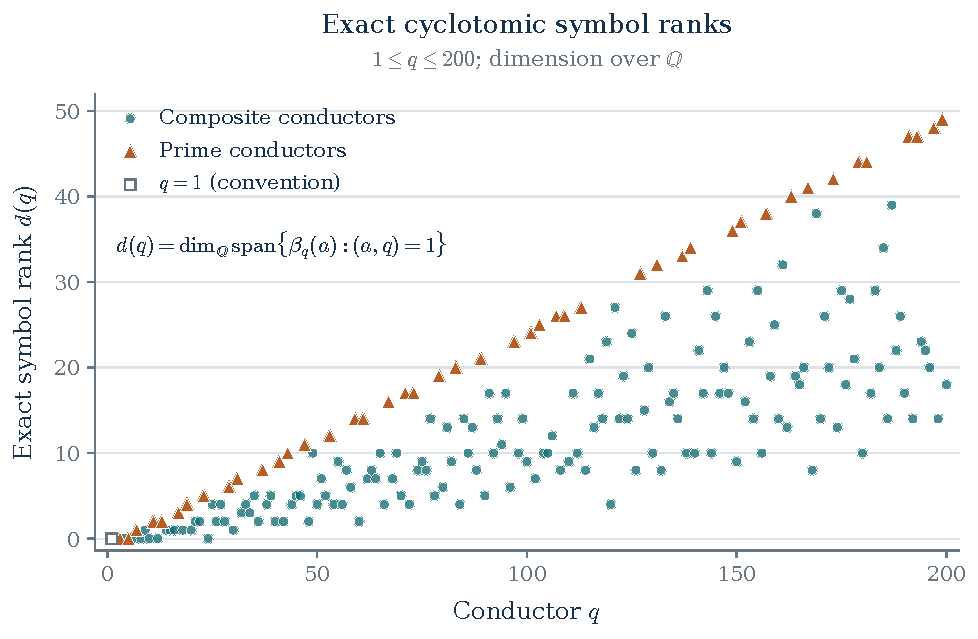
\includegraphics[width=.92\linewidth]{figures/cyclotomic_rank.pdf}
\caption{Exact ranks of the cyclotomic symbol spaces for conductors
$1\le q\le200$. The plotted values come from integer residue counts
and the proved rank formula. They are not numerical estimates of
linear independence among evaluated periods.}
\label{fig:rank}
\end{figure}

\section{Exact reduction criteria and constructive rational cores}
\label{sec:reduction}

The two cyclotomic pieces in \eqref{eq:delta-xi} cannot cancel across
coprime conductors. This needs a norm on the \emph{individual exterior
factors}; averaging an exterior symbol under Galois action would not work,
because the symbols themselves are invariant.

\begin{lemma}[Separation by normalized field norms]\label{lem:norm}
Let $(p,q)=1$ and regard both symbols in
$\Lambda^2\Acal(K)$, $K=\Q(\zeta_{pq})$. Then
\begin{equation}\label{eq:norm-separate}
 \beta_q(p)-\beta_p(q)\in\Lambda^2\Acal(\Q)
 \quad\Longleftrightarrow\quad
 \beta_q(p)=\beta_p(q)=0.
\end{equation}
\end{lemma}
\begin{proof}
Let $E=\Q(\zeta_p)$ and define the linear normalized norm
\[
 N_p:\Acal(K)\longrightarrow\Acal(E),\qquad
 \cl u\longmapsto\frac{\cl{\operatorname{Norm}_{K/E}(u)}}{[K:E]}.
\]
It fixes the vectors from $E$. The fields $\Q(\zeta_p)$ and
$\Q(\zeta_q)$ are linearly disjoint over $\Q$. In each summand of
$\beta_q(p)$, the two factors are Galois conjugate in $\Q(\zeta_q)$,
so $N_p$ sends them to the same rational vector. Hence
\[
 (\Lambda^2N_p)\beta_q(p)=0,
 \qquad(\Lambda^2N_p)\beta_p(q)=\beta_p(q).
\]
The analogous statements hold with $p,q$ exchanged. If the difference
equals a rational wedge $W$, applying $\Lambda^2N_p$ gives
$W=-\beta_p(q)$. Applying $\Lambda^2N_q$ to this equality gives $W=0$,
and both symbols vanish. The converse is immediate. The conventions
for conductor $1$ or $2$ make the same argument valid in the degenerate
field cases.
\end{proof}

\begin{theorem}[Complete formal reduction criterion]\label{thm:reduction}
For coprime positive integers $p,q$, the following are equivalent:
\begin{enumerate}
\item $\xi_{p/q}$ has a formal rational-dilogarithm reduction.
\item $\beta_q(p)=\beta_p(q)=0$.
\item $p^2\equiv\pm1\pmod q$ and $q^2\equiv\pm1\pmod p$.
\end{enumerate}
Moreover, $\xi_{p/q}$ has a formal logarithmic reduction if and only if
$p=1$ or $q=1$.
\end{theorem}
\begin{proof}
If $\xi_{p/q}$ is represented by rational dilogarithms, its differential
is a rational wedge. Equations \eqref{eq:delta-xi} and
\eqref{eq:norm-separate} imply (2). Conversely, if (2) holds, the
differential is $-\cl p\wedge\cl q$. By \eqref{eq:bloch-facts} choose
$\eta\in\Pcal(\Q)$ with this differential. Then
$\xi_{p/q}-\eta$ is a Galois-invariant Bloch-group element and hence
zero. The equivalence with (3) is Theorem~\ref{thm:kernel}.

For the last assertion, a normalized norm to $\Q$ sends every
$\beta$-summand to zero on the exterior square. Thus
$\partial\xi_{p/q}=0$ implies $\cl p\wedge\cl q=0$. If $p,q>1$
are coprime, their prime-exponent vectors have disjoint nonempty supports,
and their wedge is nonzero. If $p=1$ or $q=1$, all terms in
\eqref{eq:delta-xi} vanish; invariant Bloch descent gives the reduction.
\end{proof}

\begin{remark}[Interpretation of a failed test]
The theorem gives a necessary and sufficient condition for a certificate
in a specified algebraic calculus. A nonzero symbol is not a proof that
the corresponding real number satisfies no other numerical identity.
Such a statement would require additional information about the kernel
of period evaluation. In particular, the theorem should not be restated
as an unconditional transcendence theorem.
\end{remark}

\subsection{Checking the boundary formula directly}

Because the reduction criterion depends on \eqref{eq:delta-xi}, it is
useful to audit that formula algebraically. The finite evaluation uses
the formal summand
\[
 f(\alpha,\beta)=
 \left[\frac{\beta}{\beta-1}\right]
 -\left[\frac{\alpha-\beta}{1-\beta}\right],
\]
summed over $\alpha^p=1$, first over nontrivial $q$th roots $\beta$, and
then with the analogous sum over nontrivial $p$th roots subtracted.
Terms with $\alpha=1$ or $\alpha=\beta$ have zero differential and
are set aside before taking multiplicative logarithms. For the remaining
roots of unity $\alpha,\beta$, put
$A=\cl{1-\alpha}$, $B=\cl{1-\beta}$,
$C=\cl{\alpha-\beta}$. Away from the terms $[0],[1]$, which contribute
zero, direct expansion gives
\[
 \partial f(\alpha,\beta)=-C\wedge A+C\wedge B+B\wedge A.
\]
The differential of the subtracted summand is antisymmetric under
$\alpha\leftrightarrow\beta$, so that sum has zero differential.
In the first sum use
\[
 \prod_{\substack{\beta^q=1\\\beta\ne1}}(\alpha-\beta)
 =\frac{\alpha^q-1}{\alpha-1},\qquad
 \prod_{\substack{\alpha^p=1\\\alpha\ne1}}(\beta-\alpha)
 =\frac{\beta^p-1}{\beta-1}.
\]
The first two wedge terms then give $-\beta_p(q)$ and $\beta_q(p)$.
The last gives $\cl q\wedge\cl p$. This proves
\eqref{eq:delta-xi} independently of any finite-field cocycle claim.

\subsection{A recurrence parametrization of the reducible pairs}

The congruence criterion has an elementary arithmetic description that
connects it to the golden-ratio ladder thread of the repository.

\begin{theorem}[Quadratic recurrence families]\label{thm:recurrences}
Apart from $(1,1)$, all coprime pairs $1\le p<q$ satisfying
\eqref{eq:pair-intro} are exactly the adjacent pairs in the following
three families. Their union need not be disjoint.
\begin{enumerate}
\item For each integer $h\ge2$,
      $u_0=1$, $u_1=h$, $u_{j+1}=h u_j-u_{j-1}$.
\item $u_0=1$, $u_1=2$, $u_{j+1}=3u_j-u_{j-1}$.
\item For each integer $h\ge1$,
      $u_0=1$, $u_1=h$, $u_{j+1}=h u_j+u_{j-1}$,
      retaining pairs in increasing order.
\end{enumerate}
The first family has both square congruences $+1$, the second both
$-1$, and the third permits opposite signs, with the usual coincidences
of signs modulo $1$ or $2$.
\end{theorem}
\begin{proof}
Suppose $1<a<b$ and write
$a^2\equiv s\pmod b$, $b^2\equiv t\pmod a$ with $s,t\in\{\pm1\}$.
Set
\[
 c=\frac{a^2-s}{b}.
\]
Then $1\le c<a$, $(c,a)=1$, and the new pair $(c,a)$ satisfies the same
conditions with signs $(t,s)$. Indeed $bc\equiv-s\pmod a$ implies
$c^2\equiv b^{-2}\equiv t\pmod a$, while $a^2\equiv s\pmod c$.
This gives a strictly descending process.

If $s=t$, the positive integer
$h=(a^2+b^2-s)/(ab)$ is preserved under descent and satisfies
$b=h a-c$. For $s=1$, the terminal pair is $(1,h)$ with $h\ge2$.
For $s=-1$, a terminal pair $(1,b)$ has $b\mid2$, so it is $(1,1)$
or $(1,2)$ and the invariant is $h=3$.

If $s=-t$, the positive integer
$h=(b^2-a^2-t)/(ab)$ is preserved and satisfies $b=h a+c$.
The terminal pairs are seeds $(1,h)$, with the terminal $(1,2)$ also
lying in the $h=1$ sequence $1,1,2,3,5,\ldots$. Reversing descent gives
the three displayed recurrences. Conversely their preserved quadratic
identities, or the same recurrence step in reverse, verify both
congruences and coprimality at every stage.
\end{proof}

For example, the second family is $1,2,5,13,34,\ldots$, the odd-index
Fibonacci numbers. The first family with $h=3$ is
$1,3,8,21,55,\ldots$, and the third with $h=3$ is
$1,3,10,33,109,\ldots$. This is an arithmetic parametrization of
\emph{which} rational arguments admit formal reduction, not an assertion
that all their logarithmic correction terms are already tabulated.

\subsection{An explicit rational-dilogarithm core}

\begin{theorem}[A short core with a boundary certificate]\label{thm:core}
For every pair satisfying Theorem~\ref{thm:reduction}, one can produce
a rational combination $C_{p/q}$ of symbols $[z]$, $0<z<1$, such that
\[
 \partial C_{p/q}=-\cl p\wedge\cl q,
 \qquad \xi_{p/q}-C_{p/q}=0\quad\hbox{in }\Pcal(K).
\]
The following recursion suffices for $1\le p<q$:
\begin{enumerate}
\item If $p=1$, use $C_{p/q}=0$.
\item If $q=p+1$, use $C_{p/q}=[p/q]$.
\item Otherwise choose $s\in\{\pm1\}$ with $q\mid p^2-s$, put
      $c=(p^2-s)/q$, and use
\begin{equation}\label{eq:core-recursion}
 C_{p/q}=C_{c/p}+
 \begin{cases}
 -\tfrac12[1-p^{-2}],&s=1,\\
 \tfrac12[p^2/(p^2+1)],&s=-1.
 \end{cases}
\end{equation}
\end{enumerate}
Put $C_{1/1}=0$. For $p>q$, negate the core for $q/p$.
After the consecutive-pair shortcut,
the number of terms is $O(\log\max(p,q))$.
\end{theorem}
\begin{proof}
The first two cases have the required differential. In the last case
$cq=p^2-s$. Direct calculation gives
\begin{align*}
 -\tfrac12\partial[1-p^{-2}]
   &=-\cl p\wedge\cl q-\cl p\wedge\cl c &&(s=1),\\
 \tfrac12\partial[p^2/(p^2+1)]
   &=-\cl p\wedge\cl q-\cl p\wedge\cl c &&(s=-1).
\end{align*}
Adding $\partial C_{c/p}=-\cl c\wedge\cl p$ leaves the required
$-\cl p\wedge\cl q$. Descent terminates by the previous theorem.
Both $C_{p/q}$ and $\xi_{p/q}$ are invariant; their difference lies in
the Bloch group and vanishes by \eqref{eq:bloch-facts}.

For the length bound, the $h=2$ minus recurrence consists of consecutive
integers and is handled in one step. Every remaining minus recurrence
has $h\ge3$ and grows by a factor greater than $2$ after its seed.
Each plus recurrence grows at least as fast as the Fibonacci recurrence.
Thus the number of descent steps is logarithmic in the larger input.
\end{proof}

\begin{center}
\begin{tabular}{ll}
\toprule
Argument & A rational-dilogarithm core for $F(p/q)-F(1)$\\
\midrule
$2/5$ & $\tfrac12\Li_2(4/5)$\\
$3/8$ & $-\tfrac12\Li_2(8/9)$\\
$4/17$ & $\tfrac12\Li_2(16/17)$\\
$5/13$ & $\tfrac12\Li_2(4/5)+\tfrac12\Li_2(25/26)$\\
$10/33$ & $\tfrac12\Li_2(9/10)-\tfrac12\Li_2(99/100)$\\
\bottomrule
\end{tabular}
\end{center}
In this table the difference between $F(p/q)-F(1)$ and the displayed
core is a combination of logarithm products and $\pi^2$. The core
algorithm certifies the dilogarithm part; it does not yet print the full
logarithmic correction. Constructing that correction efficiently and
with a complete branch certificate is a further research task.

\begin{corollary}[A lower bound for a family of formal values]
Fix $q\ge3$ and choose one positive numerator representing each
nontrivial inverse pair in $G_q$. The corresponding $d(q)$ elements
$\xi_{a/q}$ are linearly independent modulo rational dilogarithms.
\end{corollary}
\begin{proof}
Take a common cyclotomic field for all numerators and $q$, and apply the
exterior square of its normalized norm to $\Q(\zeta_q)$. The
numerator-conductor symbols disappear and the denominator symbols
$\beta_q(a)$ remain. If their combination were a rational wedge, the
normalized norm to $\Q$ would kill it, so it would be zero. The chosen
$\beta_q(a)$ are independent by Theorem~\ref{thm:kernel}.
\end{proof}

\section{Complete classification and evaluations of \texorpdfstring{$J(2/q)$}{J(2/q)}}
\label{sec:J}

Define
\[
 S(n)=\sum_{k=1}^{n-1}\log^2\!\left(2\sin\frac{\pi k}{n}\right),
 \qquad S(1)=0,
 \qquad \phi=\frac{1+\sqrt5}{2}.
\]
The reciprocal-integer identity, obtainable by pairing conjugate roots
in the finite dilogarithm formula, is
\begin{equation}\label{eq:F1n}
 F(1/n)-F(1)
 =-\frac{(n-1)(3n-2)}{24n}\pi^2-\frac12 S(n),\qquad n\ge1.
\end{equation}
All logarithms here are real logarithms of positive algebraic numbers.

\begin{theorem}[Complete formal classification]\label{thm:J-class}
For integers $q\ge2$:
\begin{enumerate}
\item $J(2/q)$ has a formal logarithmic reduction exactly when
      $q\in\{2,3,5\}$ or $4\mid q$.
\item It has a formal rational-dilogarithm reduction exactly when
      $q\in\{2,3,5,6,10\}$ or $4\mid q$.
\end{enumerate}
In every positive case the evaluations below give the corresponding
analytic identity.
\end{theorem}
\begin{proof}
First suppose $q$ is odd. Applying \eqref{eq:delta-xi} to
\eqref{eq:J-F} at $x=2/q$, the numerator symbols at conductors
$1,2,4$ vanish and the rational wedges cancel. Thus the boundary is
\[
 \beta_q(4)-2\beta_q(2).
\]
Put $g=2\in G_q$. By Theorem~\ref{thm:kernel}, this vanishes exactly
when $g$ has order at most $2$. To check the assertion directly, an
element of order $3$ gives $\beta(g^2)-2\beta(g)=-3\beta(g)$; order
$4$ gives $-2\beta(g)$; for order at least $5$, the two relevant
inverse pairs are distinct. Hence vanishing is equivalent to
$4\equiv\pm1\pmod q$, or $q=3,5$. A rational wedge cannot remove a
nonzero combination of these symbols, since the normalized norm to
$\Q$ kills the combination and fixes rational wedges. This proves
both classifications for odd $q$.

If $4\mid q$, all three arguments $4/q,2/q,1/q$ in
\eqref{eq:J-F} are reciprocal integers. Equation \eqref{eq:F1n}
gives a logarithmic reduction.

The remaining case is $q=2m$ with $m$ odd. Its boundary is
\begin{equation}\label{eq:J-even-boundary}
 \beta_m(2)-\cl2\wedge\cl m.
\end{equation}
For $m=1$ it is zero. For $m>1$, applying the normalized norm to
$\Q$ gives the nonzero rational wedge $-\cl2\wedge\cl m$;
there is no formal logarithmic reduction. Rational dilogarithms are
allowed exactly when $\beta_m(2)=0$, equivalently $m=3,5$.
Invariant Bloch descent supplies the stated formal reductions.
\end{proof}

\subsection{All positive evaluations}

The isolated cases are
\begin{align}
 J(1)&=\tfrac12\log^22,\label{eq:J1}\\
 J(2/3)&=-\frac{\pi^2}{144}+\frac34\log^22,\label{eq:J23}\\
 J(2/5)&=\frac{11\pi^2}{240}+\frac34\log^22-2\log^2\phi,
 \label{eq:J25}\\
 J(1/3)&=\frac{\pi^2}{9}+\frac12\log^22-\frac12\log^23
          -\Li_2(1/3),\label{eq:J13}\\
 J(1/5)&=\frac{7\pi^2}{60}+\frac12\log^22-\frac14\log^25
          -\log^2\phi-\frac12\Li_2(1/5).\label{eq:J15}
\end{align}
For all even $m\ge2$, the infinite family is
\begin{equation}\label{eq:J-even-family}
 \boxed{\displaystyle
 J(1/m)=\frac{\pi^2(m^2-2)}{48m}
       +S(m)-\frac12S(m/2)-\frac12S(2m).}
\end{equation}
Thus \eqref{eq:J-even-family} evaluates $J(2/q)$ for every multiple
$q$ of $4$, without a dilogarithm term.

\begin{proof}[Derivation of the evaluations]
Equation \eqref{eq:J1} follows by integrating
$\log(1+t)/(1+t)$. For \eqref{eq:J-even-family}, substitute
\eqref{eq:F1n} at $n=m/2,m,2m$ in \eqref{eq:J-F}. The constant
$F(1)$ cancels; the polynomial coefficient simplifies to
$m/48-1/(24m)$, yielding the formula.

The small odd cases are obtained from the finite root-of-unity
dilogarithm formula and the reflection, duplication, and Landen
relations. For clarity, the two fractional $F$ evaluations needed in
the calculation can be taken as
\begin{align*}
 F(2/3)-F(1)
  &=\frac{\pi^2}{36}+\log^22-\frac34\log^23-\Li_2(1/3),\\
 F(2/5)-F(1)
  &=\tfrac12\Li_2(4/5)-\frac{\pi^2}{5}
    +\log^2\!\left(2\sin\frac\pi5\right)
    +\log^2\!\left(2\sin\frac{2\pi}5\right)
    +\log2\log(2/5).
\end{align*}
The second is the previously known evaluation \cite{RZ}; the first
follows by using $\cot^2(\pi/3)=1/3$ in the $F(2/q)$ sum and
$\Li_2(-1/3)=2\Li_2(1/3)-\pi^2/6+\tfrac12\log^23$.
Substitution in \eqref{eq:J-F}, together with \eqref{eq:F1n} and
the two standard functional equations
\begin{align*}
 F(x)+F(1/x)&=2F(1)+\tfrac12\log^2x
                 -\frac{\pi^2(x-1)^2}{6x},\\
 F(x)-F(x+1)-F(x/(x+1))&=-F(1)+\Li_2(1/(1+x)),
\end{align*}
gives \eqref{eq:J23}--\eqref{eq:J15}. Reflection of
$\Li_2(4/5)$ supplies the $\Li_2(1/5)$ in \eqref{eq:J15}.
All manipulations use arguments in $(0,1)$ or the real negative axis,
so no unstated complex logarithm branches are involved.
\end{proof}

The first member of \eqref{eq:J-even-family} is particularly useful
for auditing the earlier claim:
\begin{equation}\label{eq:Jhalf}
 J(1/2)=\frac{\pi^2}{48}+\frac14\log^22.
\end{equation}
The complete classification proves a precise replacement for the
unsupported numerical ``if and only if'' in the draft. It also shows
that the distinction between logarithms and rational dilogarithms is
real at the level of the boundary: the cases $q=6,10$ have a nonzero
rational wedge, even though their cyclotomic obstruction vanishes.

\section{A positive measure and certified remainder bounds}
\label{sec:measure}

The analytic part begins with a representation already obtained by
Radchenko and Zagier \cite[\S7.3]{RZ}. We derive its consequences
explicitly, keeping signs and normalizations visible. Put
\begin{equation}\label{eq:G}
 G(x)=-F(x)-\frac{\zeta(2)}{2x},\qquad
 \Lam(u)=\sum_{m=1}^{\infty}\sigma_{-1}(m)e^{-2\pi m u},
 \qquad \sigma_{-1}(m)=\sum_{d\mid m}\frac1d.
\end{equation}
Expanding a geometric series gives
\[
 \Lam(u)=\sum_{n=1}^{\infty}\frac1{n(e^{2\pi n u}-1)}.
\]
Binet's digamma integral, followed by a positive change of variables
and Tonelli's theorem, yields
\begin{equation}\label{eq:Stieltjes}
 G(x)=2\int_0^\infty\frac{u\Lam(u)}{x^2+u^2}\,du
     =\int_0^\infty\frac{d\mu(s)}{x^2+s},
 \qquad d\mu(s)=\Lam(\sqrt{s})\,ds.
\end{equation}
Thus $y\mapsto G(\sqrt y)$ is a Stieltjes transform of a positive
measure with a positive density on $(0,\infty)$.

\begin{lemma}[Explicit moments]\label{lem:moments}
Every nonnegative moment exists, and
\begin{equation}\label{eq:moments}
 \mu_j:=\int_0^\infty s^j\,d\mu(s)
 =\frac{2\Gamma(2j+2)\zeta(2j+2)\zeta(2j+3)}
        {(2\pi)^{2j+2}}
 =\frac{|B_{2j+2}|}{2j+2}\zeta(2j+3).
\end{equation}
\end{lemma}
\begin{proof}
Substitute $s=u^2$, integrate each positive exponential term, and use
$\sum_m\sigma_{-1}(m)m^{-w}=\zeta(w)\zeta(w+1)$ for $w>1$.
Euler's formula for the even zeta values gives the second equality.
\end{proof}

Define the approximation and its first omitted term by
\begin{equation}\label{eq:FN}
 F_N(x)=-\frac{\zeta(2)}{2x}
         -\sum_{j=0}^{N-1}\frac{(-1)^j\mu_j}{x^{2j+2}},
 \qquad T_N(x)=\frac{\mu_N}{x^{2N+2}},
 \qquad N\ge0.
\end{equation}
The empty sum for $N=0$ is zero. The series is asymptotic and divergent;
we will work with its exact finite remainder.

\begin{theorem}[Signed remainder and three-moment bounds]
\label{thm:remainder}
For $x>0$ and $N\ge0$,
\begin{align}
 F(x)-F_N(x)&=(-1)^{N+1}R_N(x),\label{eq:signed-R}\\
 R_N(x)&=x^{-2N}\int_0^\infty\frac{s^N}{x^2+s}\,d\mu(s)>0,
 \label{eq:R-exact}\\
 R_N(x)+R_{N+1}(x)&=T_N(x).\label{eq:R-sum}
\end{align}
Set
\[
 A=\frac{\mu_{N+1}}{\mu_Nx^2},\qquad
 B=\frac{\mu_{N+2}}{\mu_Nx^4}.
\]
Then the strict bounds
\begin{equation}\label{eq:three-moment}
 \frac1{1+A}<\frac{R_N(x)}{T_N(x)}
       <1-\frac{A^2}{A+B}<1
\end{equation}
hold. In particular, two consecutive truncations bracket $F(x)$.
\end{theorem}
\begin{proof}
The finite geometric identity
\[
 \frac1{x^2+s}
 =\sum_{j=0}^{N-1}\frac{(-s)^j}{x^{2j+2}}
    +\frac{(-1)^Ns^N}{x^{2N}(x^2+s)}
\]
gives \eqref{eq:signed-R}--\eqref{eq:R-exact}, and multiplying the
remainder integrand by $1+s/x^2$ gives \eqref{eq:R-sum}.

Under the probability measure $s^N\,d\mu(s)/\mu_N$ let $U=s/x^2$.
Then $R_N/T_N=\E(1+U)^{-1}$, $\E U=A$, and $\E U^2=B$.
Strict Jensen convexity gives the lower bound. Cauchy--Schwarz gives
\[
 \E\frac{U}{1+U}\ \E\bigl(U(1+U)\bigr)\ge(\E U)^2,
\]
so $\E(1+U)^{-1}\le1-A^2/(A+B)$. Both inequalities are strict
because the measure has a nonconstant positive-density support.
\end{proof}

For interval computation, an equivalent and useful form is
\begin{align}
 L_N(x)&=\frac{x^{-2N}\mu_N^2}{x^2\mu_N+\mu_{N+1}},\nonumber\\
 L_N(x)&<R_N(x)<T_N(x)-L_{N+1}(x).
 \label{eq:interval-R}
\end{align}
It uses only three adjacent moments, and hence only rational
Bernoulli numbers and odd zeta values. No oscillatory integral is needed.

\subsection{An exact rational certification scheme}

For integer $s\ge2$, integer $M\ge2$, and $J\ge1$, Euler--Maclaurin
gives
\begin{align}
 Z_{M,J}(s)
 &=\sum_{n=1}^{M-1}n^{-s}
   +\frac{M^{1-s}}{s-1}+\frac1{2M^s}\nonumber\\
 &\quad+\sum_{j=1}^{J-1}
 \frac{B_{2j}}{(2j)!}(s)_{2j-1}M^{-s-2j+1},\label{eq:EM}\\
 |\zeta(s)-Z_{M,J}(s)|
 &\le
 \frac{|B_{2J}|}{(2J)!}(s)_{2J-1}M^{-s-2J+1}.
 \label{eq:EM-bound}
\end{align}
Here $(s)_k$ is a rising factorial. A direct positive-kernel proof
is useful because it fixes the endpoint convention in this bound.
The partial fraction expansion of the hyperbolic cotangent gives
\[
 k(t):=\frac1{1-e^{-t}}-\frac1t-\frac12
       =2t\sum_{n\ge1}\frac1{t^2+(2\pi n)^2},\qquad t>0.
\]
Expand each denominator through $J-1$ terms by the finite geometric
identity. After summing, the result is
\[
 k(t)=\sum_{j=1}^{J-1}\frac{B_{2j}}{(2j)!}t^{2j-1}
           +\varepsilon_J(t),\qquad
 |\varepsilon_J(t)|
 \le\frac{|B_{2J}|}{(2J)!}t^{2J-1}.
\]
Indeed the remainder before summing is
$(-1)^{J-1}2t^{2J-1}/
((2\pi n)^{2J-2}((2\pi n)^2+t^2))$, whose magnitude is bounded
by replacing the last denominator by $(2\pi n)^2$.
Integrate against $t^{s-1}e^{-Mt}/\Gamma(s)$, using
\[
 \sum_{n=M}^\infty n^{-s}
 =\frac1{\Gamma(s)}
       \int_0^\infty\frac{t^{s-1}e^{-Mt}}{1-e^{-t}}\,dt.
\]
This proves \eqref{eq:EM}--\eqref{eq:EM-bound}, including the
first-omitted-term bound, rather than assuming a truncation-sign rule.
Related sharper Hurwitz-zeta remainder bounds are discussed in
\cite{Nemes}.

All quantities in \eqref{eq:EM}--\eqref{eq:EM-bound} are rational.
Combining their enclosing intervals with
\eqref{eq:moments}, \eqref{eq:FN}, and \eqref{eq:interval-R} yields
exact rational endpoints for $F(x)$ when $x$ is rational.
The code uses interval operations with integer numerators and
denominators throughout; decimal endpoints are rounded outward only
for display.

\begin{center}
\begin{tabular}{rrl}
\toprule
$x$ & $N$ & Certified width of the interval for $F(x)$, at most\\
\midrule
$2$  & $6$  & $4.18751510340\times10^{-7}$\\
$4$  & $12$ & $4.88272699850\times10^{-13}$\\
$8$  & $25$ & $2.15471915709\times10^{-24}$\\
$16$ & $50$ & $1.10232929493\times10^{-46}$\\
\bottomrule
\end{tabular}
\end{center}
These are reproducible certificates, not estimates based on the number
of floating-point digits. The file
\texttt{data/rational\_intervals.json} contains the complete exact
endpoints. The parameters here are $M=J=48$; no optimality of that
computational choice is asserted.

\subsection{Classical Stieltjes consequences}

The representation also settles the qualitative approximation question
without any new special-function identity.

\begin{proposition}[Determinacy and positive rational approximation]
\label{prop:Stieltjes}
The measure $\mu$ is uniquely determined by its moments. Gaussian
quadrature for $\mu$ produces lower bounds that are rational functions of $y$ for
$G(\sqrt y)$, $y>0$; Gauss--Radau quadrature with a prescribed node at
$0$ produces rational upper bounds. These bounds converge pointwise to
$G(\sqrt y)$ as their orders tend to infinity.
\end{proposition}
\begin{proof}
Stirling's formula in \eqref{eq:moments} gives
$\mu_j^{-1/(2j)}\sim\pi e/j$. Thus the Stieltjes Carleman sum
diverges, which implies determinacy. The quadrature error signs follow
from the alternating derivatives of $(y+s)^{-1}$: Gaussian
quadrature has a positive even-order remainder, while the Radau rule
with left endpoint $0$ has a negative odd-order remainder.
For convergence, the discrete positive quadrature measures have the
same total mass and, eventually, every fixed finite set of moments as
$\mu$. A first-moment bound gives tightness; higher moment bounds give
uniform integrability of each fixed power. Every subsequential weak
limit therefore has all the moments of $\mu$ and must equal $\mu$ by
determinacy. Integration of the bounded continuous function
$(y+s)^{-1}$ proves the claim. These are standard Stieltjes and Pad\'e
consequences; see \cite{Simon}.
\end{proof}

The value of the proposition here is practical: it explains why
positive rational approximations are available even in parameter
regimes where an asymptotic series is not an efficient evaluator.
An effective convergence rate for this particular measure remains
a separate problem.

\section{Uniform sharp asymptotics at the optimal scale}
\label{sec:sharp}

The scale $N\sim\pi x$ can be located from the ratio of consecutive
moments. To obtain the error constant and its corrections, it is
more efficient to convert the exact remainder into gamma expectations.
Write
\begin{equation}\label{eq:gamma-notation}
 a=2\pi x,\quad K=2N+2,\quad r=K-a=2\delta+2,\quad
 \delta=N-\pi x.
\end{equation}
Let $T$ have gamma density $t^{K-1}e^{-t}/\Gamma(K)$ on $(0,\infty)$,
and define
\[
 E_K(c)=\E\frac1{1+(T/c)^2},\qquad
 w_m=\sigma_{-1}(m)m^{-K},\qquad
 Z_K=\sum_{m\ge1}w_m=\zeta(K)\zeta(K+1).
\]

\begin{lemma}[Exact gamma mixture]\label{lem:gamma-mixture}
For all $x>0$ and $N\ge0$,
\begin{equation}\label{eq:gamma-mixture}
 R_N(x)=\frac{2\Gamma(K)}{a^K}\sum_{m=1}^\infty w_m E_K(ma),
 \qquad T_N(x)=\frac{2\Gamma(K)}{a^K}Z_K.
\end{equation}
For $K\ge4$,
\begin{equation}\label{eq:frequency-tail}
 0<Z_K-1\le4\,2^{-K}.
\end{equation}
\end{lemma}
\begin{proof}
In each positive exponential summand of \eqref{eq:R-exact}, written
in the variable $u=\sqrt s$, substitute $t=2\pi m u$. Collecting
powers gives \eqref{eq:gamma-mixture}. For the tail, use
$\sigma_{-1}(m)\le m$ and
\[
 \sum_{m\ge2}m^{1-K}
 \le 2^{1-K}+\frac{2^{2-K}}{K-2}\le4\,2^{-K}.
\]
\end{proof}

The arithmetic terms $m\ge2$ therefore do not affect any algebraic
coefficient in the optimal-scale expansion. They do, however, move
the exact transition point by an exponentially small amount; this
effect is treated separately in Section~\ref{sec:arithmetic}.

\subsection{Gamma moments and a uniform remainder mechanism}

Let $f(v)=(1+v^2)^{-1}$ and $H=(T-a)/a$. The local Taylor expansion is
\[
 f(1+H)=\frac12-\frac H2+\frac{H^2}4-\frac{H^4}8
                +\frac{H^5}8-\frac{H^6}{16}+\cdots,
\]
and the moments are exactly
\begin{equation}\label{eq:gamma-moments}
 \E H^\ell
 =a^{-\ell}\sum_{j=0}^{\ell}
       \binom{\ell}{j}(-a)^{\ell-j}(a+r)_j.
\end{equation}
This is an algebraic coefficient algorithm, not a fit to numerical data.

For rigor at any fixed order $J$, Taylor-expand $f$ through degree
$2J+1$. Every derivative of $f$ is bounded on $[0,\infty)$, so the
absolute remainder is bounded by a constant times $|H|^{2J+2}$.
The centered gamma cumulants are $K(j-1)!$ in orders $j\ge2$.
Consequently each centered even moment of order $2J+2$ is a polynomial
in $K$ of degree at most $J+1$. Translating the center from $K$ to
$a=K-r$, with $r$ bounded, gives
\[
 \E|H|^{2J+2}=O_J(a^{-J-1})
\]
uniformly on each compact interval of $r$. This proves the required
uniform remainder after taking expectations. In particular,
\begin{align}
 2E_K(a)
 &=1+\frac{1/2-r}{a}
   +\frac{(r^2+r)/2-3/4}{a^2}
   +\frac{-3r^2/2+r/4+13/8}{a^3}\nonumber\\
 &\quad-\frac{4r^4-16r^3-66r^2+74r+59}{16a^4}
   +O_D(a^{-5}).\label{eq:gamma-expansion}
\end{align}
The subscript $D$ signifies that the constant may depend on a fixed
bound for $|r|$; the same convention will be used for $\delta$.

The classical shifted Stirling expansion \cite[\S5.11.8]{DLMF} is
\begin{equation}\label{eq:shifted-Stirling}
 \frac{\Gamma(a+r)}{a^{a+r}}
 \sim \sqrt{2\pi}\,a^{-1/2}e^{-a}
 \exp\left(\sum_{j=1}^\infty
 \frac{(-1)^{j+1}B_{j+1}(r)}{j(j+1)a^j}\right).
\end{equation}
It is uniform for $r$ in compact sets. Combining its rigorous finite
forms with the gamma-moment argument proves the following theorem.

\begin{theorem}[Complete optimal-scale expansion]\label{thm:sharp}
For each fixed $D>0$ and each integer $J\ge0$, there are explicitly
computable rational polynomials $C_j(\delta)$ such that, uniformly
for integers $N\ge0$ with $|N-\pi x|\le D$,
\begin{equation}\label{eq:all-orders}
 R_N(x)=\frac{e^{-2\pi x}}{\sqrt{x}}
 \left(\sum_{j=0}^{J}\frac{C_j(\delta)}{(2\pi x)^j}
       +O_{D,J}(x^{-J-1})\right).
\end{equation}
The first three are
\begin{align}
 C_0(\delta)&=1,\nonumber\\
 C_1(\delta)&=2\delta^2+\delta-\frac5{12},\label{eq:C1}\\
 C_2(\delta)&=2\delta^4+\frac23\delta^3-\frac{10}3\delta^2
                         -\frac7{12}\delta+\frac{205}{288}.
 \label{eq:C2}
\end{align}
Moreover, $R_N(x)/T_N(x)\longrightarrow1/2$ uniformly in that regime.
\end{theorem}
\begin{proof}
Use \eqref{eq:gamma-moments} to expand $2E_K(a)$, multiply by
\eqref{eq:shifted-Stirling}, and put $r=2\delta+2$.
The frequency tail \eqref{eq:frequency-tail} is smaller than every
power of $a^{-1}$. The leading factor is
$\sqrt{2\pi}\,a^{-1/2}e^{-a}=x^{-1/2}e^{-2\pi x}$.
For an explicit check of the first two coefficients, put
$g_1=B_2(r)/2$ and $g_2=-B_3(r)/6$. Before substituting for $r$ they are
\[
 g_1+\tfrac12-r,\qquad
 \tfrac12g_1^2+g_2+g_1(\tfrac12-r)
                       +\tfrac12(r+r^2)-\tfrac34.
\]
These simplify to \eqref{eq:C1}--\eqref{eq:C2}. The ratio assertion
follows directly from \eqref{eq:gamma-mixture}, since $E_K(a)\to1/2$
and $Z_K\to1$.
\end{proof}

The leading constant is therefore exactly $1$. Replacing the true
remainder by the first omitted term loses a factor of $2$ at the
optimal scale. The three-moment bounds also approach this factor:
there $A\to1$ and $B\to1$, so both sides of
\eqref{eq:three-moment} tend to $1/2$.

The program \texttt{code/truncation\_coefficients.py} generates
$C_j$ symbolically using rational polynomial operations and
Bernoulli polynomials. The theorem's bounded-$\delta$ condition is
essential to the stated uniformity. A growing window, for example
$N-\pi x$ of order $\sqrt{x}$, requires a different scaling.

\section{The exact best cutoff and its transitions}
\label{sec:cutoff}

An asymptotic nearest-integer rule is useful, but it cannot determine
the best cutoff arbitrarily close to a transition. The positive
measure supplies an exact answer.

\begin{theorem}[Unique transitions and global minimizers]
\label{thm:transitions}
For every $N\ge0$, there is a unique $x_N>0$ such that
$R_N(x_N)=R_{N+1}(x_N)$. The sequence $x_N$ is strictly increasing
and tends to infinity. With $x_{-1}=0$, the index $N$ is a global
minimizer of $R_j(x)$, $j\ge0$, exactly when
\begin{equation}\label{eq:exact-cutoff}
 x_{N-1}\le x\le x_N.
\end{equation}
There are exactly two adjacent minimizing indices at an endpoint
and exactly one elsewhere on $x>0$. An exact transition equation is
\begin{equation}\label{eq:transition-integral}
 x_N^2\int_0^\infty\frac{s^N}{x_N^2+s}\,d\mu(s)=\frac{\mu_N}2.
\end{equation}
\end{theorem}
\begin{proof}
Put $y=x^2$ and
$M_N(y)=\int s^N(y+s)^{-1}\,d\mu(s)$.
Strict Cauchy--Schwarz gives
\[
 M_{N+1}(y)^2<M_N(y)M_{N+2}(y).
\]
Hence $R_N=y^{-N}M_N(y)$ is strictly log-convex as a sequence in
$N$, and its consecutive ratios are strictly increasing.
The recurrence $M_{N+1}=\mu_N-yM_N$ gives
\begin{equation}\label{eq:ratio-R}
 \frac{R_{N+1}(x)}{R_N(x)}
 =\frac{\mu_N}{yM_N(y)}-1.
\end{equation}
By dominated convergence,
$yM_N(y)=\int s^N y/(y+s)\,d\mu(s)$ increases continuously and
strictly from $0$ to $\mu_N$ as $y$ increases from $0$ to infinity.
The ratio in \eqref{eq:ratio-R} thus decreases continuously from
infinity to $0$, proving the unique transition and
\eqref{eq:transition-integral}.

Strict increase of the ratios in $N$ forces $x_{N+1}>x_N$.
For fixed $y$, the moment ratios $M_{N+1}/M_N$ tend to infinity.
Indeed, if their increasing sequence were bounded by $B$, the
moments would be at most $M_0B^N$, contradicting positive mass on
an interval strictly to the right of $B$. This also proves
$x_N\to\infty$ and existence of a global minimum. The strict ratio
monotonicity now gives \eqref{eq:exact-cutoff} and the assertions
about ties.
\end{proof}

To expand the transition, let $\alpha_K$ be the unique positive root of
\begin{equation}\label{eq:alpha}
 E_K(\alpha_K)=\frac12,
\end{equation}
and write $\beta_K=2\pi x_N$ for $K=2N+2$. The full transition is
the unique root of
\begin{equation}\label{eq:Phi}
 \Phi_K(a):=\sum_{m\ge1}w_m\left(E_K(ma)-\frac12\right)=0.
\end{equation}
The symbols $\alpha_K,\beta_K$ in this analytic section are real
numbers; the subscript and argument distinguish $\beta_K$ from the
cyclotomic symbol $\beta_q(a)$.

\begin{theorem}[Algebraic transition expansion]\label{thm:transition-exp}
Put $b=K-\tfrac12=2N+\tfrac32$. As $N\to\infty$,
\begin{equation}\label{eq:transition-exp}
 \alpha_K=b+\frac3{8b}-\frac1{b^2}
                +\frac{407}{128b^3}+O(b^{-4}).
\end{equation}
The same expansion holds for $\beta_K=2\pi x_N$, and the two
quantities have identical expansions to every algebraic order.
\end{theorem}
\begin{proof}
The gamma law gives $T/K\to1$ in probability. Evaluating at $a=cK$
shows that both roots have $a/K\to1$. More precisely, substitution
of $a=K+C$ for fixed constants on either side of $C=-1/2$
in \eqref{eq:gamma-expansion} brackets both roots for large $K$;
the frequency tail does not change these opposite signs. Therefore
$r=K-a$ is bounded at the roots, and the uniform expansion applies.

Solve $2E_K(a)=1$ from \eqref{eq:gamma-expansion} to obtain
\[
 r=\frac12-\frac3{8a}+\frac1{a^2}
                    -\frac{425}{128a^3}+O(a^{-4}).
\]
For example, putting $r=1/2+q_1/a+q_2/a^2+q_3/a^3$ gives
successively $q_1=-3/8$, $q_2=1$, $q_3=-425/128$.
Since $\partial_a[2E_K(a)]$, with $K$ fixed, is
$1/K+O(K^{-2})$ near the root (see \eqref{eq:shift-derivative}),
a residual of order
$a^{-j-1}$ locates the root to order $a^{-j}$. Thus the formal
inversion has the asserted error control. Reexpressing it in
$b=K-1/2$ yields \eqref{eq:transition-exp}. Finally, the perturbing
tail in \eqref{eq:Phi} is $O(2^{-K})$, while its derivative is of
order $1/K$; it changes the root by $O(K2^{-K})$. This proves the
last assertion.
\end{proof}

To leading order, choose the integer nearest to $\pi x-1/4$.
The exact prescription remains \eqref{eq:exact-cutoff}; no rounding
formula with an unspecified remainder resolves every near-tie case.

\section{An arithmetic displacement beyond all algebraic orders}
\label{sec:arithmetic}

The comparison in this section is between two exactly defined
transition points. Subtracting a finite approximation such as
$b+3/(8b)-1/b^2$ would leave an algebraic error much larger than
the effect we want to measure.

\begin{theorem}[First arithmetic shift]\label{thm:arithmetic-shift}
For every $K=2N+2\ge2$, the full transition satisfies
$0<\beta_K<\alpha_K$. As $K\to\infty$,
\begin{equation}\label{eq:arithmetic-shift}
 \boxed{\displaystyle
 \beta_K-\alpha_K
 =-\frac9{10}K2^{-K}
  \left(1+O(K^{-1})+O((2/3)^K)\right).}
\end{equation}
Equivalently, with $x_N^{(1)}=\alpha_K/(2\pi)$,
$x_N-x_N^{(1)}$ has leading term $-9K2^{-K}/(20\pi)$.
\end{theorem}
\begin{proof}
The function $E_K(c)$ is strictly increasing in $c$. At
$a=\alpha_K$, the $m=1$ term of \eqref{eq:Phi} vanishes, while
every $m\ge2$ term is positive. Hence $\Phi_K(\alpha_K)>0$.
Since $\Phi_K$ is strictly increasing, its root lies below $\alpha_K$.

For the coefficient, $\alpha_K=K+O(1)$ and gamma concentration
with its second-moment bound gives
\[
 E_K(2\alpha_K)=\frac45+O(K^{-1}).
\]
Also $w_2=(3/2)2^{-K}$ and $\sum_{m\ge3}w_m=O(3^{-K})$.
Therefore
\begin{equation}\label{eq:shift-numerator}
 \Phi_K(\alpha_K)
 =\frac9{20}2^{-K}
   \left(1+O(K^{-1})+O((2/3)^K)\right).
\end{equation}
Differentiation under the expectation gives
\[
 E_K'(a)=\frac1a\,\E h(T/a),\qquad
 h(v)=\frac{2v^2}{(1+v^2)^2}.
\]
On a bounded neighborhood of $K$, $h(1)=1/2$ and a
second-moment expansion yield
$E_K'(a)=(2K)^{-1}(1+O(K^{-1}))$.
For any $m$, the derivative of $E_K(ma)$ with respect to $a$ is
$a^{-1}\E h(T/(ma))$, and $0<h\le1/2$. Thus
\begin{equation}\label{eq:shift-derivative}
 \Phi_K'(a)=\frac1{2K}\bigl(1+O(K^{-1})+O(2^{-K})\bigr)
\end{equation}
uniformly in that neighborhood. In particular it has a positive
lower bound of order $K^{-1}$. The mean value theorem first gives
$\beta_K-\alpha_K=O(K2^{-K})$ and then, using
\eqref{eq:shift-numerator}--\eqref{eq:shift-derivative}, gives
\eqref{eq:arithmetic-shift}.
\end{proof}

The constant has a transparent decomposition:
\[
 \frac9{10}
 =\underbrace{\frac32}_{\text{divisor weight at }m=2}
  \underbrace{\left(\frac45-\frac12\right)}_{\text{kernel gap}}
  \bigg/\underbrace{\frac12}_{\text{scaled derivative}}.
\]
It records the second Lambert frequency, rather than a correction to
the Stirling expansion.

\begin{remark}[A transferable positive-mixture calculation]
The same argument applies to a positive exponential mixture with
frequencies $1,\rho,\ldots$, $\rho>1$, and coefficients $c_1,c_\rho>0$.
If its higher-frequency Dirichlet tail is $o(\rho^{-K})$, the
corresponding normalized transition displacement is
\[
 -\frac{c_\rho}{c_1}\frac{\rho^2-1}{\rho^2+1}
                 K\rho^{-K}(1+o(1)).
\]
This follows by replacing the kernel limit $4/5$ by
$\rho^2/(1+\rho^2)$ in the proof. It is a useful extension of the
calculation, rather than a claim to a new general method of
exponentially improved asymptotics; see \cite[\S2.11]{DLMF} for
the broader established theory.
\end{remark}

\subsection{The periodic correction to the best attainable error}

\begin{corollary}[Integer-cutoff oscillation]\label{cor:lattice}
Uniformly for real $x\to+\infty$,
\begin{equation}\label{eq:minimum-R}
 \min_{N\ge0}R_N(x)
 =\frac{e^{-2\pi x}}{\sqrt{x}}
 \left[
 1+\frac{2\dist(\pi x-\tfrac14,\Z)^2-\tfrac{13}{24}}{2\pi x}
 +O(x^{-2})
 \right].
\end{equation}
The numerator of the first correction ranges from $-13/24$ to
$-1/24$.
\end{corollary}
\begin{proof}
Complete the square in \eqref{eq:C1}:
$C_1(\delta)=2(\delta+1/4)^2-13/24$.
The exact transition expansion shows that the optimizing index
differs from a nearest integer to $\pi x-1/4$ only within
$O(x^{-1})$ of a tie phase. There the squared distances for the
two competing integers differ by $O(x^{-1})$; after multiplication
by $(2\pi x)^{-1}$ this contributes only $O(x^{-2})$.
The bounded-$\delta$ uniformity of Theorem~\ref{thm:sharp} completes
the proof, including arbitrarily close approaches to transition points.
\end{proof}

\begin{figure}[!tb]
\centering
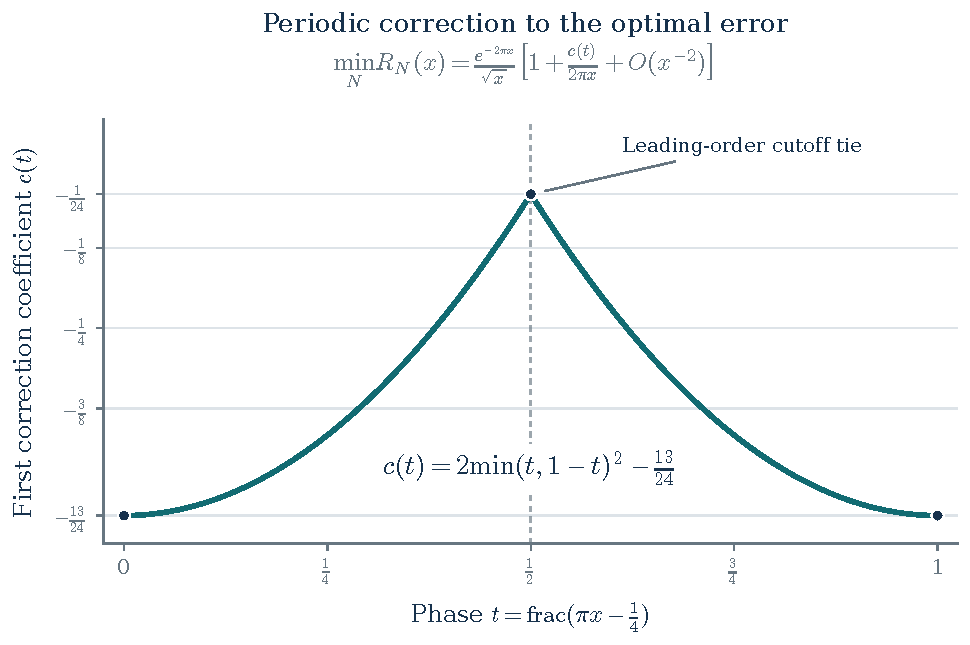
\includegraphics[width=.92\linewidth]{figures/optimal_correction.pdf}
\caption{The explicit first correction in \eqref{eq:minimum-R}, as
a function of the fractional part of $\pi x-1/4$. This plots a proved
coefficient function, not fitted numerical data. The two endpoint
phases represent the same point of the unit circle.}
\label{fig:optimal-correction}
\end{figure}

\section{Corrections proposed for the source drafts}
\label{sec:corrections}

The proposals below refer to the pinned snapshot in
Section~\ref{sec:scope}. The machine-readable file
\texttt{data/proposed\_corrections.json} records exact paths, anchors,
evidence, and the distinction between false statements, missing
proofs, and synchronization of an already repaired formula.
No source file in the repository has been changed by this package.

\subsection{The denominator-only collapse criterion}

The reports \texttt{herglotz-arithmetic-study} and
\texttt{herglotz-rational-values}, at
\texttt{prop:collapse}, assert a reduction criterion depending only
on whether the prime divisors of $q$ belong to $\{2,3,5\}$.
The necessity fails even for actual analytic reductions:
\[
 F(1/7)-F(1)=-\frac{19\pi^2}{28}-\frac12S(7)
\]
is logarithmic, by \eqref{eq:F1n}. The core at $4/17$ supplies a
nontrivial-numerator example with a rational dilogarithm.
As a formal criterion, the proposed sufficiency also fails:
$F(2/9)-F(1)$ has nonzero cyclotomic symbol, since
$4\not\equiv\pm1\pmod9$.

\paragraph{Proposed replacement.}
Replace the proposition by Theorem~\ref{thm:reduction}, including its
definition of formal reduction. The proof must depend on both
numerator and denominator. Remove any inference from bounded PSLQ
failure to numerical nonreducibility. The rational core table and
recurrence algorithm give constructive positive examples outside the
claimed denominator set.

\subsection{The missing infinite family of logarithmic \texorpdfstring{$J$}{J}-values}

The same reports state that $J(2/q)$ is logarithmic exactly for
$q=3,5$, and that reciprocal-integer $J$-values always retain
dilogarithms. The explicit value \eqref{eq:Jhalf} already
contradicts both assertions. In fact every $q$ divisible by $4$
belongs to a logarithmic family.

\paragraph{Proposed replacement.}
Use Theorem~\ref{thm:J-class}, with the analytic formulas
\eqref{eq:J1}--\eqref{eq:J-even-family}. Include the endpoint
$q=2$. Preserve the distinction between the extra rational-dilogarithm
cases $q=6,10$ and the pure logarithmic cases. The positive identities
are unconditional numerical evaluations; the necessity statements
are explicitly statements about the formal calculus.

\subsection{The undefined middle term in the derivative sum}
\label{sec:derivative-correction}

In the derivative law of the Herglotz reports, the displayed sum
\[
 \sum_{k=1}^{q-1}\cot(2\pi k/q)\Cl_2(2\pi k/q)
\]
contains the undefined factor $\cot\pi$ when $q$ is even. An
additional $-\log2$ is then mentioned separately, leaving two
incompatible possible conventions.
Define instead
\begin{equation}\label{eq:Wstar}
 W^*(q)=\sum_{\substack{1\le k<q\\k\ne q/2}}
       \cot(2\pi k/q)\Cl_2(2\pi k/q).
\end{equation}
The exclusion has no effect when $q$ is odd. The corrected formula is
\begin{equation}\label{eq:derivative-correct}
 \frac2qF'(2/q)-(1+\log2)
 =\frac{q^2-4}{24q}\pi^2+W^*(q)
                  -\mathbf1_{2\mid q}\log2.
\end{equation}
To see exactly which term is at issue, use
$\Cl_2'(\theta)=-\log(2\sin(\theta/2))$ near $\theta=\pi$.
Then $\Cl_2(\pi+h)=-h\log2+O(h^3)$ and
$\cot(\pi+h)=h^{-1}+O(h)$, giving
\[
 \lim_{\theta\to\pi}\cot\theta\,\Cl_2(\theta)=-\log2.
\]
Thus an alternative valid convention is to include this continuous
extension in $W(q)$ and omit the separate correction. It must be
counted exactly once. Formula \eqref{eq:derivative-correct} is the
corresponding specialization of the rational derivative formula in
\cite[Proposition~4]{RZ}.

For example, $W^*(4)=0$, and
\begin{equation}\label{eq:Fprimehalf}
 F'(1/2)=2+\frac{\pi^2}4.
\end{equation}
This also refutes the reports' unrestricted assertion that the
derivative expression never becomes elementary.

\paragraph{Coefficient fields.}
For the nonsingular terms one has
\[
 \cot(2\pi k/q)=i\,\frac{\zeta_q^{2k}+1}{\zeta_q^{2k}-1}.
\]
Accordingly a uniformly valid real coefficient field is
$\Q(\zeta_{\operatorname{lcm}(4,q)})^+$, which need not be
$\Q(\zeta_q)^+$. Membership of an individual coefficient in a
smaller field does not decide whether a whole evaluated Clausen
combination admits another expression. Replace the claimed
field-membership equivalence with this field containment
and whatever exact identities are actually proved.

\subsection{A counterexample in the inspected 2020 preprint}
\label{sec:preprint-counterexample}

The final paragraph of \S7.2, printed page~16 of the inspected
18-page 2020 preprint \cite{RZ}, displays the untwisted identity
\begin{equation}\label{eq:printed-finite-identity}
 \beta_p(n)=\beta_p(n+1)+\beta_p\!\left(\frac n{n+1}\right).
\end{equation}
For its stated exterior-square symbol, this identity is false.
Take $p=7$, $n=2$. Since $2/3=3$ in $\mathbb F_7$ and the class
of $3$ is inverse to that of $2$ modulo sign,
\[
 \beta_7(3)=-\beta_7(2).
\]
Equation \eqref{eq:printed-finite-identity} would therefore imply
$3\beta_7(2)=0$. But $2^2=4$ is neither $1$ nor $-1$ modulo $7$,
so Theorem~\ref{thm:kernel} proves $\beta_7(2)\ne0$.

There is also a small exact matrix certificate. In the regular basis
of sign classes $1,2,3$, the image of the defect under the coordinate
model $\beta_7(a)\mapsto P_a-P_{a^{-1}}$ is
\begin{equation}\label{eq:p7-defect}
 \begin{pmatrix}
 0&3&-3\\-3&0&3\\3&-3&0
 \end{pmatrix}\ne0.
\end{equation}
Its entries are integers; no numerical logarithm independence test
enters this counterexample.

\paragraph{Proposed correction and version scope.}
Withdraw the untwisted identity as printed, or supply a corrected
coefficient action or quotient together with a proof. This article
does not guess what a missing action should be. The definition of
$\beta$ and the boundary formula \eqref{eq:delta-xi} remain valid;
the latter was independently derived in Section~\ref{sec:reduction}.
The separately published 2023 journal version was not inspected in
this audit. The correction is therefore specifically to the inspected
2020 preprint, and must not be attributed to an unchecked version.

\subsection{Cubic subfields and regulator normalization}
\label{sec:Stark-correction}

The report \texttt{herglotz-stark-regulators} calls a degree-three
polynomial field over $\Q$ a Hilbert or ring class field of a real
quadratic field. These are different fields. Let $L/\Q$ be the
non-Galois cubic field, $K$ its quadratic resolvent, and $H=LK$
its normal closure. Then $[H:\Q]=6$ and $[H:K]=3$. The class-field
description, when established, concerns $H/K$; the cubic regulator
in the displayed polynomial table is $R_L$.

A leading-$L$-value identity follows from classical Artin formalism
and the analytic class-number formula, with a factor that the report
suppresses.

\begin{proposition}[The cubic leading coefficient]
\label{prop:cubic-L}
Let $L$ be a totally real non-Galois cubic field with normal closure
$H$ and quadratic resolvent $K$. For either nontrivial character
$\chi$ of $\Gal(H/K)\simeq C_3$, use the primitive Artin
$L$-function with all its finite Euler factors. Then
\begin{equation}\label{eq:cubic-L}
 L_K(s,\chi)=\frac{\zeta_L(s)}{\zeta(s)},\qquad
 \lim_{s\to0}s^{-2}L_K(s,\chi)=h_LR_L.
\end{equation}
\end{proposition}
\begin{proof}
The induced representation
$\operatorname{Ind}_{C_3}^{S_3}\chi$ is the standard
two-dimensional representation of $S_3$. The permutation
representation on the three embeddings of $L$ is its direct sum
with the trivial representation. Artin induction, including the
ramified Euler factors, proves the quotient identity
\cite{Cogdell}. Since $L$ is totally real of degree three, it has
unit rank $2$ and two roots of unity. The class-number formula at
zero gives
$\zeta_L(s)=-(h_LR_L/2)s^2+O(s^3)$, whereas $\zeta(0)=-1/2$.
Division proves the leading coefficient \cite[Theorem~3.1.2]{Dasgupta}.
\end{proof}

Thus the coefficient is $R_L$ only after $h_L=1$ has been
established. This proposition neither proves the report's other
fitted Herglotz--regulator identities nor upgrades a numerical fit to
a theorem. It replaces the unsupported appeal to a general Stark
theorem with the precise classical identity that is needed here.

\paragraph{An exact class-number certificate at discriminant $257$.}
Use the report's polynomial $f(X)=X^3-2X^2-3X+1$ and a root
$\alpha$. Its squarefree discriminant is $257$, so
$\mathcal O_L=\Z[\alpha]$. The cubic Minkowski bound is
$(2/9)\sqrt{257}<4$. Modulo $2$, the polynomial is irreducible,
so there is no prime ideal of norm $2$. Modulo $3$ it factors as
$(X-1)(X^2+2X+2)$, with the quadratic irreducible. The unique
prime of norm $3$ is principal, since
$\operatorname{Norm}_{L/\Q}(\alpha-1)=3$.
Every ideal class therefore has a principal representative of norm
at most $3$, proving $h_L=1$. This agrees with the database record
\cite{LMFDB257}, and does not rely on that record as a proof.

\paragraph{The conductor convention at discriminant $257$.}
Here the cubic character has actual conductor $1$, although it can
be represented with modulus $2$. This also follows from the
conductor-discriminant identity
$\operatorname{disc}(L)=\operatorname{disc}(K)
\operatorname{Norm}_{K/\Q}(\mathfrak f_\chi)$:
both discriminants are $257$.
The prime $2$ splits in $K=\Q(\sqrt{257})$.
The irreducible reduction of $f$ modulo $2$ shows that Frobenius
is a $3$-cycle, so the character values at the two primes above
$2$ are $\omega,\omega^2$. Removing those Euler factors changes
the function to
\begin{equation}\label{eq:imprimitive}
 L_{\mathrm{omitting}\ 2}(s,\chi)
 =(1+2^{-s}+2^{-2s})L_{\mathrm{primitive}}(s,\chi).
\end{equation}
Its leading coefficient is $3h_LR_L$, not $h_LR_L$.
Any computational comparison using ray-class software must state
which Euler factors were included. A difference of this kind should
not be explained by an unspecified unit index.

\subsection{Adjacent CM and polylogarithm corrections}

These are targeted repairs, rather than a second full research thread.
Some were already corrected in a later article or a report addendum;
the source bodies still need to be synchronized.

\begin{enumerate}
\item In \texttt{polygamma-complex-arguments-cm-lattices}, for
      $s\ge1$ and $a\notin\Z$, the bilateral identity is
\[
 \sum_{m\in\Z}(m+a)^{-s-1}
 =\frac{(-1)^{s+1}\psi^{(s)}(a)+\psi^{(s)}(1-a)}{s!}.
\]
The omitted sign matters at even $s$. Split the positive and
negative halves of the absolutely convergent series to prove it.

\item At discriminant $-15$, the real expression must use
      $\Rea G_4((1+i\sqrt{15})/4)$, or its conjugate average.
      The main-body use of the raw complex value is incompatible
      with a real right side. This repair is already present in
      the report's correction addendum and the associated article.
      The normalized algebraic number
      $(29+12\sqrt5)/44$ has norm $1/16$; $121$ is the norm of
      its numerator.

\item Replace assertions that $E_4$ or $E_6$ do not exist at special
      lattices by the correct vanishing-value statements.
      For the equianharmonic point $\rho=e^{2\pi i/3}$,
      $G_4(\rho)=0$; for the square point $i$, $G_6(i)=0$.
      The modular forms themselves exist.

\item In \texttt{polylog-polygamma-bridge}, specify the weight
      parity: the standard Clausen component is antisymmetric in
      the angle at even weight and symmetric at odd weight.
      The real part of $\Li_{2m+1}(e^{i\theta})$ is not an
      antisymmetric component.

\item The claimed necessity of the crystallographic-angle rule
      needs a separate independence theorem. The supplied
      character decompositions prove identities and certain
      sufficient reductions; they do not prove that all other
      numerical reductions are impossible. Similarly, unsuccessful
      PSLQ searches in the CM article do not establish an
      irrationality statement or an exact algebraic degree.
      Replace categorical claims by the proved decomposition and
      an explicitly bounded computational observation.
\end{enumerate}

The original repository already distinguishes a number of conjectural
claims in its README. The proposed corrections preserve that useful
distinction and apply it consistently to the specific formulas above.

\section{Research questions and a concrete continuation program}
\label{sec:questions}

The results resolve the relation problem for the individual
$\beta_q$-families and the formal classification of the indicated
values. They leave several sharply defined problems. We separate
constructive next steps from questions that require substantially
new mathematics.

\subsection{Constructive algebra and exact identities}

\begin{enumerate}
\item \textbf{Recover the full logarithmic remainder.}
      The core recursion certifies the rational dilogarithm part
      but does not print its logarithmic correction. Construct an
      algorithm that returns both a finite five-term certificate
      and the exact coefficients of all logarithm products and
      $\pi^2$, with a branch certificate on the positive real
      axis. The first useful benchmark is a fully explicit family
      for adjacent terms of each recurrence in
      Theorem~\ref{thm:recurrences}. The objective is a constructive
      identity, not another numerical fit.

\item \textbf{Minimize the rational core.}
      Our length bound is logarithmic in the input height.
      Determine the minimal number of rational arguments needed
      after allowing five-term moves, duplication, and shared
      prime support. Does the recurrence construction have
      asymptotically optimal length in a precisely specified
      certificate model? Distinguish term count, coefficient
      height, and bit complexity.

\item \textbf{Relations involving several conductors.}
      For a prescribed finite set of rational arguments, compute
      the full kernel of their combined boundary map, including
      the distribution relations between proper cyclotomic
      subfields. The single-conductor kernel and normalized norms
      provide exact blocks and projections. What additional
      relations appear when the conductors share prime factors?
      A finite implementation should output a rational basis of
      certificates and record its ambient coefficient field.

\item \textbf{Repair the finite-field relation with explicit data.}
      Identify the correct coefficient module and action, if any,
      behind \eqref{eq:printed-finite-identity}. Require an identity
      that survives the $p=7,n=2$ certificate and whose relation
      to the analytic three-term equation is proved. This is a
      question about a different or enriched algebraic structure;
      the untwisted equation in the present symbol space has
      already been disproved.
\end{enumerate}

\subsection{Periods, derivatives, and higher weight}

\begin{enumerate}[resume]
\item \textbf{The kernel of numerical period evaluation.}
      What additional conjecture would promote the formal
      obstruction in Theorem~\ref{thm:reduction} to a numerical
      nonreduction result? Formulate the period algebra and its
      permitted logarithmic constants explicitly. Even a restricted
      injectivity theorem for a fixed conductor would be a major
      strengthening. A nonzero exterior symbol alone does not
      settle this question.

\item \textbf{A symbol theory for rational derivatives.}
      The rational higher derivatives are already known to
      involve cyclotomic polylogarithms \cite[\S4]{RZ}.
      Develop exact relation modules with the correct coefficient
      fields, weight parity, and lower-weight products, starting
      from the derivative sum \eqref{eq:Wstar}. Can a positive
      character matrix detect all relations in an appropriate
      higher-weight boundary, or does the exterior-square
      argument rely on a feature special to weight two?

\item \textbf{Higher polylogarithm ladders from quadratic recurrences.}
      The reduction pairs connect naturally to Fibonacci and
      golden-ratio ladders. Determine which recurrence identities
      lift to higher Bloch complexes, keeping motivic or formal
      relations separate from evaluated real identities. The
      first goal should be explicit weight-three boundary
      calculations, with all product terms retained.
\end{enumerate}

\subsection{Sharp approximation and arithmetic asymptotics}

\begin{enumerate}[resume]
\item \textbf{A growing cutoff window.}
      Obtain a uniform expansion when $N-\pi x$ grows with $x$,
      especially the transition scale $O(\sqrt{x})$. The
      bounded-offset proof gives exact moments but not the right
      uniform normalization in that window. Determine a range
      and an explicit error bound, rather than extending
      \eqref{eq:all-orders} without qualification.

\item \textbf{Several exponentially small frequencies.}
      Theorem~\ref{thm:arithmetic-shift} isolates $m=2$ against an
      exact $m=1$ reference. Define exact references including
      $m\le M$ and determine the displacement contributed by
      $m=M+1$. At higher exponential orders, nonlinear
      interactions of previous displacements may coincide with
      arithmetic frequencies. A complete expansion should state
      how such terms are ordered and give a uniform tail estimate.

\item \textbf{Effective Stieltjes approximation.}
      Find quantitative rates for the Gaussian/Radau rational
      bounds associated with $d\mu(s)=\Lam(\sqrt s)\,ds$.
      Analyze the relevant orthogonal polynomials and Hankel
      determinants, then compare the cost with optimally
      truncated Bernoulli series and exact rational certificates.
      Determinacy proves convergence, but does not supply an
      efficient a priori rate.

\item \textbf{Complex sectors and Stokes behavior.}
      Extend the exact remainder analysis away from the positive
      axis, locating the sectors where the positive-real
      estimates have useful analogues and describing what
      replaces positivity. Relate the resulting terminants and
      Stokes transitions to established exponentially improved
      asymptotics, rather than treating them as unexplained
      numerical effects.
\end{enumerate}

\subsection{Regulators and formal verification}

\begin{enumerate}[resume]
\item \textbf{Complete the regulator certificates.}
      For each proposed real-quadratic evaluation, identify the
      cubic subfield, its normal closure, conductor, class number,
      primitive Euler factors, and the exact partial-zeta
      combination. Then derive the coefficients multiplying
      $h_LR_L$ from the class-group character decomposition.
      The leading-$L$-value formula \eqref{eq:cubic-L} is proved;
      the additional fitted Herglotz identities require their
      own certificates.

\item \textbf{Formalize the finite and analytic proof components.}
      A realistic first stage for ProveIt is the finite inverse-pair
      kernel model, the CRT rank calculation, the recurrence
      descent, the prime-exponent wedge certificates, and the
      rational interval arithmetic. A second stage can import
      or formalize Dirichlet nonvanishing, Bloch descent,
      Tonelli, and the gamma remainder estimates. Keeping those
      dependencies explicit avoids confusing an executable
      finite check with a formal proof of the infinite theorem.
\end{enumerate}

The most immediately implementable follow-up is the full logarithmic
certificate generator. The sharpest conceptual question is the gap
between the formal relation space and the kernel of period evaluation.
The analytic program offers a separate tractable path through
effective rational approximation and successive arithmetic
transition corrections.

\section{Reproducibility, evidence, and integration}
\label{sec:reproducibility}

The ZIP is a self-contained source package. It includes this
\LaTeX{} source and the compiled PDF, figure sources and exports,
the snapshot inventory, structured proposed corrections, exact
arithmetic certificates, and the Python programs used for the
finite and numerical checks. The bibliography is embedded in the
\texttt{.tex} file, so no external bibliography database is needed
to compile the article.

\subsection{What the checks establish}

\begin{itemize}
\item \texttt{verify\_cyclotomic.py} constructs exact regular
      permutation matrices and tests the inverse-pair relation
      model. It checks the integer root-count formula through
      $q=1000$, exact Gaussian-elimination ranks through $q=80$,
      and the complete $J(2/q)$ boundary classification through
      $q=1000$. It also prints \eqref{eq:p7-defect}.
      These finite checks support the proof; they do not replace
      the character argument for arbitrary conductor.

\item \texttt{verify\_recurrences.py} checks that all $1076$
      admissible coprime pairs with $1\le p\le q\le500$ are
      generated by the three recurrence families.
      \texttt{dilogarithm\_cores.py} checks all $2106$ admissible
      pairs up to $1000$ and their reciprocals, giving $4212$
      exact boundary checks in the prime-exponent exterior basis.
      The largest core length in this finite range is $13$,
      attained at $610/987$.

\item \texttt{verify\_J\_evaluations.py} evaluates the defining
      positive real integral independently of the finite
      dilogarithm formula. At 80-digit working precision the
      isolated evaluations and the even-$m$ family through
      $m=40$ agree to a maximum absolute residual below
      $2.1\times10^{-79}$. These are floating-point checks.

\item \texttt{verify\_truncation.py} evaluates gamma expectations
      by a special-function expression and cross-checks selected
      cases by positive-real quadrature. Its transition
      calculations attach analytic bounds for the omitted
      Dirichlet tail. Floating-point root-solving errors are
      not certified by those tail bounds; the data explicitly
      distinguish a computed truncated root from an exact root.

\item \texttt{certified\_intervals.py} is different in status:
      its interval endpoints are exact fractions obtained from
      the proved positive-kernel zeta bound and
      Theorem~\ref{thm:remainder}. It needs only the Python
      standard library. Its data are mathematical interval
      certificates, conditional only on faithful execution of
      the explicitly given exact-arithmetic algorithm.
\end{itemize}

For orientation, the numerical ratios
$-(\beta_K-\alpha_K)/((9/10)K2^{-K})$ are approximately
$0.995699$, $0.993203$, $0.996502$, $0.998249$, and $0.999125$
at $K=12,22,42,82,162$, respectively. The nonmonotone beginning
is compatible with the theorem, which asserts an asymptotic limit,
not monotonic convergence of this scaled ratio.

\subsection{A bound for numerical frequency truncation}

For $K>1$, the elementary estimate
$\sigma_{-1}(m)\le1+\log m$ gives
\begin{equation}\label{eq:numeric-tail}
 \sum_{m>M}w_m
 \le M^{1-K}\left(\frac{1+\log M}{K-1}
                         +\frac1{(K-1)^2}\right).
\end{equation}
Every omitted summand of \eqref{eq:Phi} has magnitude at most
$w_m/2$. To convert this to a root-location bound on
$a\in[K-1,K]$, $K\ge8$, use Chebyshev's inequality:
the event $K/2\le T\le3K/2$ has probability at least $1/2$.
On that event $T/a\in[1/2,2]$ and $h(T/a)\ge8/25$.
Consequently
$\Phi_K'(a)\ge4/(25K)$. If the full and truncated roots lie in
that bracket, their distance is at most $25K/8$ times the right
side of \eqref{eq:numeric-tail}. This certifies the effect of
the missing frequencies, separately from arithmetic rounding.

\subsection{Suggested repository integration}

Place the article source and PDF in the repository's article
directory, and retain the code, figures, data, and README together
in a companion subdirectory or preserve this package as a unit.
The figure paths in the source are relative. The proposed
correction records name the old source files explicitly so they
can be reviewed and applied without relying on current line numbers.
The package includes a SHA-256 manifest for the delivered artifacts.
It contains no asserted changes to the pinned upstream snapshot.

\clearpage
\phantomsection
\addcontentsline{toc}{section}{References}
\begin{thebibliography}{99}

\bibitem{RZ}
D.~Radchenko and D.~Zagier,
\emph{Arithmetic properties of the Herglotz function},
2020 preprint, arXiv:2012.15805v1.
Inspected author-hosted version:
\url{https://people.mpim-bonn.mpg.de/zagier/files/preprints/HerglotzFunction.pdf}.
Published in \emph{J. reine angew. Math.} \textbf{797} (2023), 229--253,
\url{https://doi.org/10.1515/crelle-2023-0009}.
The separate journal text was not inspected for the correction in
Section~\ref{sec:preprint-counterexample}.

\bibitem{ZagierDilog}
D.~Zagier,
\emph{The dilogarithm function},
in P.~Cartier, B.~Julia, P.~Moussa, and P.~Vanhove (eds.),
\emph{Frontiers in Number Theory, Physics, and Geometry II},
Springer, 2007, pp.~3--65.
\url{https://doi.org/10.1007/978-3-540-30308-4_1}.

\bibitem{Milnor}
J.~Milnor,
\emph{Introduction to Algebraic K-Theory},
Annals of Mathematics Studies \textbf{72},
Princeton University Press, 1971.
\url{https://doi.org/10.1515/9781400881796}.

\bibitem{Washington}
L.~C.~Washington,
\emph{Introduction to Cyclotomic Fields}, second edition,
Graduate Texts in Mathematics \textbf{83}, Springer, 1997.
\url{https://doi.org/10.1007/978-1-4612-1934-7}.

\bibitem{Sharifi}
R.~Sharifi,
\emph{Iwasawa theory}, online lecture notes, Chapter~4
(cyclotomic units and Dirichlet $L$-values).
\url{https://www.math.ucla.edu/~sharifi/notes/iwasawa-ch04.html}.
Accessed 8 October 2026.

\bibitem{DLMF}
NIST,
\emph{Digital Library of Mathematical Functions},
\S\S2.11, 5.11, and 25.15; in particular the shifted Stirling
expansion and Dirichlet nonvanishing.
\url{https://dlmf.nist.gov/}.
Accessed 8 October 2026.

\bibitem{Nemes}
G.~Nemes,
\emph{Error bounds for the asymptotic expansion of the Hurwitz
zeta function},
\emph{Proc. R. Soc. A} \textbf{473} (2017), 20170363.
\url{https://doi.org/10.1098/rspa.2017.0363};
\url{https://arxiv.org/abs/1702.05316}.

\bibitem{Simon}
B.~Simon,
\emph{The classical moment problem as a self-adjoint finite
difference operator},
\emph{Adv. Math.} \textbf{137} (1998), 82--203.
\url{https://doi.org/10.1006/aima.1998.1728};
\url{https://arxiv.org/abs/math-ph/9906008}.

\bibitem{Cogdell}
J.~W.~Cogdell,
\emph{On Artin $L$-functions}, author's expository text,
especially the induction formalism.
\url{https://math.osu.edu/~cogdell/artin-www.pdf}.

\bibitem{Dasgupta}
S.~Dasgupta,
\emph{Stark's Conjectures}, thesis, Theorem~3.1.2
(the analytic class-number formula at zero).
\url{https://sites.math.duke.edu/~dasgupta/papers/Dasguptaseniorthesis.pdf}.

\bibitem{LMFDB257}
The LMFDB Collaboration,
Number field \texttt{3.3.257.1}.
\url{https://www.lmfdb.org/NumberField/3.3.257.1}.
Accessed 8 October 2026.

\bibitem{ProveIt}
V.~Reshetnikov,
\emph{ProveIt}, \path{Analysis/Polylogarithms/docs},
pinned snapshot cited in Section~\ref{sec:scope}.
\url{https://github.com/VladimirReshetnikov/ProveIt/tree/c78c7c3dc2fc742a1af9492e47d578b3fb4e01e7/Analysis/Polylogarithms/docs}.
Exact source file inventory supplied with this article.

\end{thebibliography}
\end{document}
